\documentclass[10.9pt]{article}

\usepackage[french]{babel}
\usepackage[utf8]{inputenc}
\usepackage{fancyhdr}
\usepackage{lastpage}
\usepackage{graphicx}
\usepackage[T1]{fontenc}
\usepackage{amsmath,amssymb}
\usepackage{fullpage}
\usepackage{url}
\usepackage{xspace}
 
\usepackage{listings}
\lstset{
  morekeywords={abort,abs,accept,access,all,and,array,at,begin,body,
      case,constant,declare,delay,delta,digits,do,else,elsif,end,entry,
      exception,exit,for,function,generic,goto,if,in,is,limited,loop,
      mod,new,not,null,of,or,others,out,package,pragma,private,
      procedure,raise,range,record,rem,renames,return,reverse,select,
      separate,subtype,task,terminate,then,type,use,when,while,with,
      xor,abstract,aliased,protected,requeue,tagged,until},
  sensitive=f,
  morecomment=[l]--,
  morestring=[d]",
  showstringspaces=false,
  basicstyle=\small\ttfamily,
  keywordstyle=\bf\small,
  commentstyle=\itshape,
  stringstyle=\sf,
  extendedchars=true,
  columns=[c]fixed
}

% CI-DESSOUS: conversion des caractères accentués UTF-8 
% en caractères TeX dans les listings...
\lstset{
  literate=%
  {À}{{\`A}}1 {Â}{{\^A}}1 {Ç}{{\c{C}}}1%
  {à}{{\`a}}1 {â}{{\^a}}1 {ç}{{\c{c}}}1%
  {É}{{\'E}}1 {È}{{\`E}}1 {Ê}{{\^E}}1 {Ë}{{\"E}}1% 
  {é}{{\'e}}1 {è}{{\`e}}1 {ê}{{\^e}}1 {ë}{{\"e}}1%
  {Ï}{{\"I}}1 {Î}{{\^I}}1 {Ô}{{\^O}}1%
  {ï}{{\"i}}1 {î}{{\^i}}1 {ô}{{\^o}}1%
  {Ù}{{\`U}}1 {Û}{{\^U}}1 {Ü}{{\"U}}1%
  {ù}{{\`u}}1 {û}{{\^u}}1 {ü}{{\"u}}1%
}

%%%%%%%%%%
% TAILLE DES PAGES (A4 serré)

\setlength{\parindent}{0pt}
\setlength{\parskip}{1ex}
\setlength{\textwidth}{17cm}
\setlength{\textheight}{24cm}
\setlength{\oddsidemargin}{-.7cm}
\setlength{\evensidemargin}{-.7cm}
\setlength{\topmargin}{-.5in}

%%%%%%%%%%
% EN-TÊTES ET PIED DE PAGES

%% \pagestyle{fancyplain}
\renewcommand{\headrulewidth}{0pt}
\addtolength{\headheight}{1.6pt}
\addtolength{\headheight}{2.6pt}
\lfoot{}
\cfoot{\footnotesize\sf TPL UNIX Avancé 2014}
\rfoot{\footnotesize\sf page~\thepage/\pageref{LastPage}}
\lhead{}


%%%%%%%%%%
% TITRE DU DOCUMENT

\title{Rapport de Projet Unix Avancé\\
  ``{\em Galerie shell}'' }
\author{\textsc{Guillaume Halb (G8)} - \textsc{Pierre Thalamy (G6)}}
\date{\today}

\begin{document}

\maketitle

Nous avons implémenté, pour les deux versions du générateur
de galerie, l'ensemble des fonctionnalités indiquées dans le
sujet. Nous avons aussi choisi de ne pas mettre l'accent sur le côté esthétique
de la gallerie, car
nous avons compris que là n'était pas l'objectif direct du travail. À
l'inverse, nous avons veillé à sécuriser au maximum notre scripts et
à corriger chaque erreur que nous avons pu rencontrer au cours du
développement. \\

\section{Version séquentielle du générateur de galerie d'image}

\subsection{Structure du générateur de galerie}

Dans la version shell du générateur, nous avons organisé notre code
avec une fonction pour chaque étape de la génération :
\begin{enumerate}
  \item \lstinline!parse_args (Arguments du script)! 
    –– Parsing des arguments.
  \item \lstinline!init ()! –– Initialisation de l'arborescence
    et des variables.
  \item \lstinline!print_index_header ()! –– Écriture de l'entête HTML de
    l'index.
  \item \lstinline!generate_thumbs ()! –– Génèration de toutes les vignettes.
  \item \lstinline!include_images ()! –– Inclusion des vignettes dans
    l'index.
  \item \lstinline!print_index_footer ()! –– Fermeture du code HTML de
    l'index.
  \item \lstinline!open_gallery ()! –– Ouverture de la galerie dans le
    navigateur si l'option \lstinline!-o! est spécifiée.
\end{enumerate}

\subsection{Testing du code}
Nous avons réalisé comme demandé un panel de fichiers de test
permettant d'attester du bon fonctionnement de la galerie d'image dans
différents cas, à savoir :
\begin{itemize}
  \item Chemins des répertoires source et destination relatifs et
    absolus.
  \item Espaces dans les noms de tous fichiers et répertoires
    manipulés.
  \item Un panel de caractère spéciaux dans les noms d'images.
  \item Exécution à sec, aucun fichier ne doit être généré.
  \item Test de la verbose et modificateur \lstinline'--open'
  \item Différentes configurations de fichiers dans les répertoires
    source et destination.
\end{itemize}

\section{Version parallèle grâce au Makefile}

\subsection{Structure du Makefile}

Pour cette version du générateur, nous avons décidé d'ajouter quelques
éléments en plus que ce qui était demandé dans le sujet, à savoir la
création d'une arborescence dans le repertoire de destination, et de
ce même répertoire si il n'existait pas lors de l'appel à
make, ainsi que la compatibilité avec les fichiers portant un nom à
espace. Ceci a été fait dans un effort d'harmonisation avec l'autre
version du générateur. \\  

D'un point de vue programmation, nous avons utilisé des
\lstinline!pattern-rules! afin de générer de façon commode les
fichiers nécessaires à la galerie. Les différents appels de scripts
sont identiques à ceux fait par la version séquentielle, on obtient
donc normalement une galerie d'image semblable pour un même répertoire
source (Sauf dans le cas où ce dernier contient des images aux noms
non pris en charge par le Makefile). \\

\begin{figure}[!h]
\begin{center}
  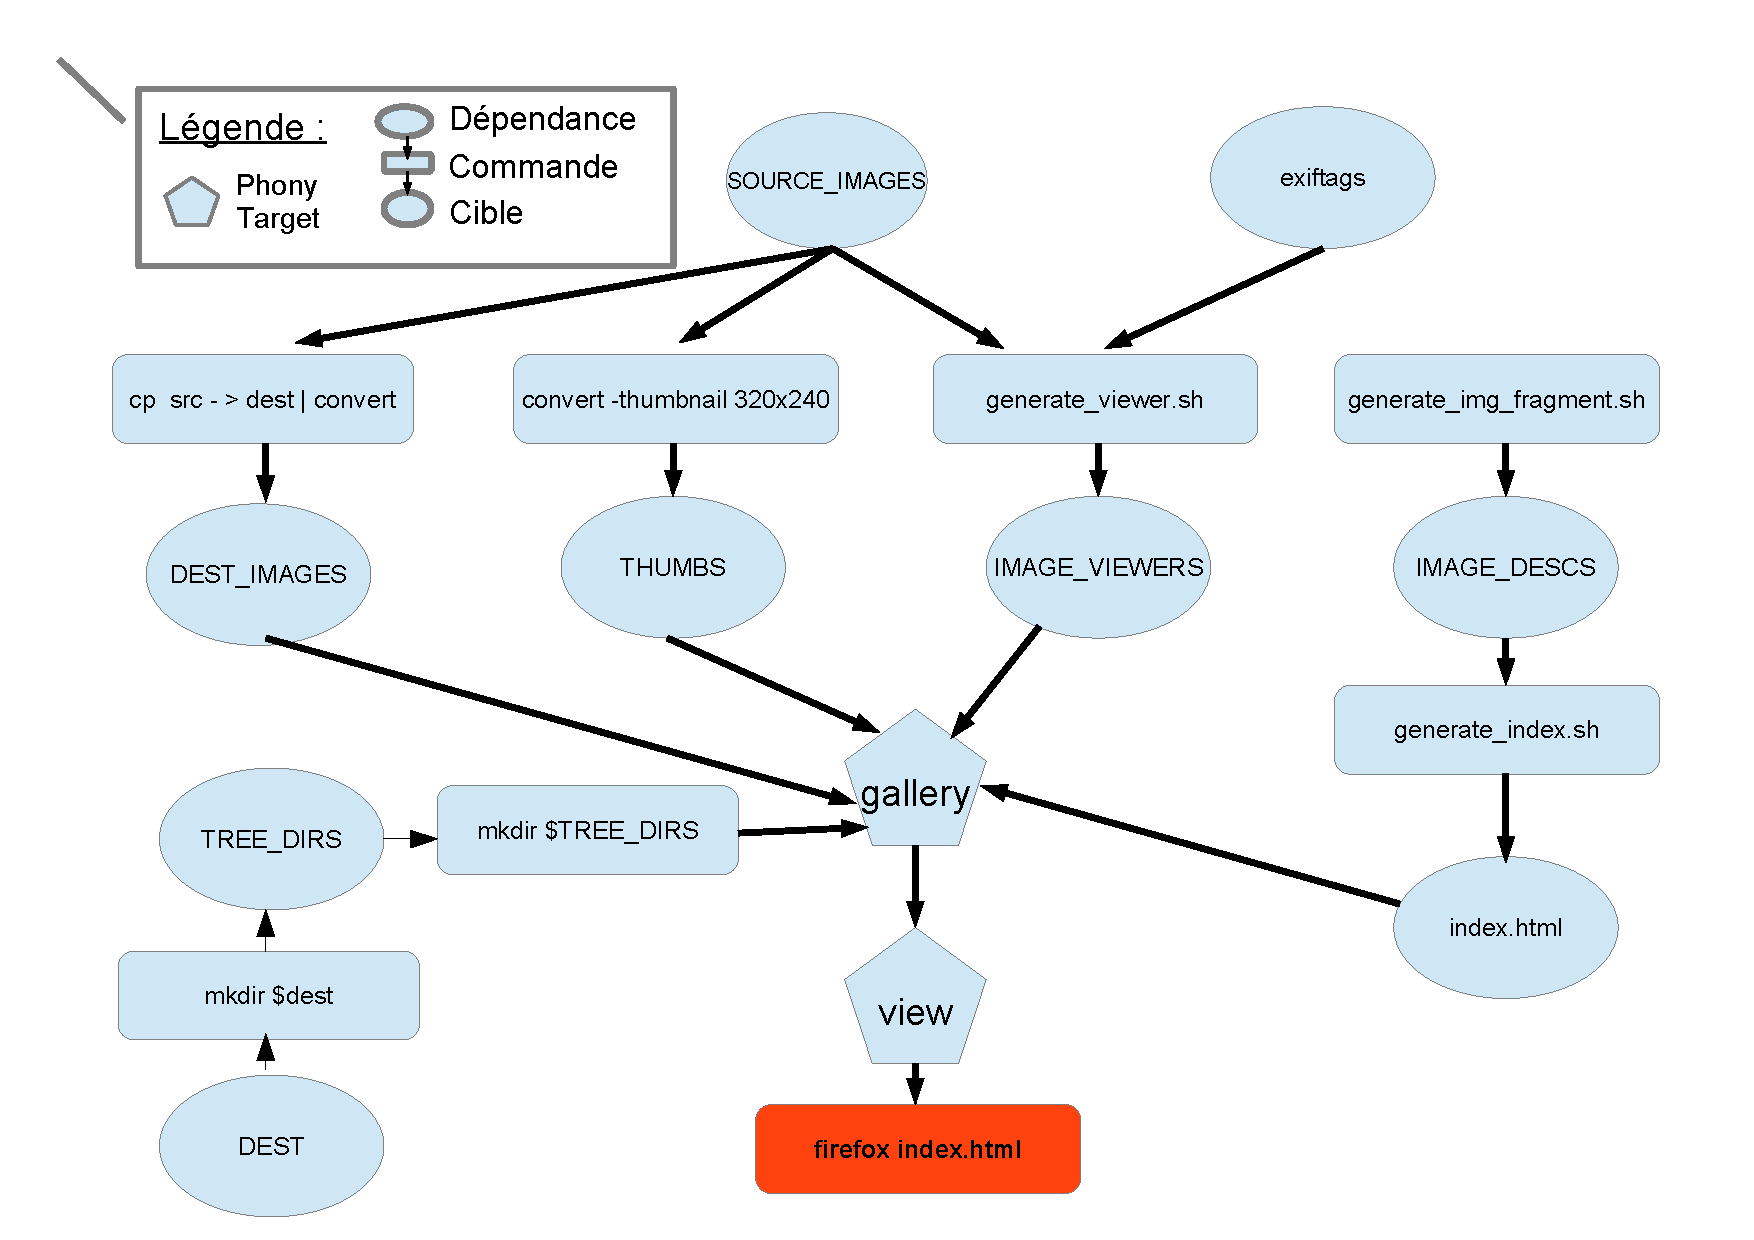
\includegraphics[width=10 cm]{makefile_graph.pdf}
  \caption{Graphe des dépendances et tâches du Makefile}
\end{center}
\label{fig:makefile_graph}
\end{figure}

La Figure~\ref{fig:makefile_graph} montre de quelle façon est
structuré notre Makefile, par soucis de clarté du schéma, les dépendances entre
\lstinline!TREE_DIR! et toutes les cibles secondaires, ainsi que les
règles de cleaning et exiftags n'ont pas été représentées.

\subsection{Analyse de l'efficacité du parallélisme}

Nous avons effectué des mesures de performance de la génération de
galerie avec divers degrés de parallélisme \lstinline!N! 
et 15 ou 100 images. Nos
résultats sont observable en Figure~\ref{fig:time_graph}. 
Quelque soit le nombre d'images, sur la machine ayant effectué les
tests, on obtient un minimum à \lstinline!N = 7! processus en
parallèle. Il semblerait que l'efficacité du parallélisme croît
avec \lstinline!N! jusqu'à ce que ce dernier soit égale au nombre de
threads maximal (en fonction du nombre de cœurs et HyperThreading) 
que la machine peut exécuter simultanément. Au delà de ce nombre, nous
supposons que c'est l'ordonnancement devant être mis en place qui influe
négativement sur l'efficacité du parallélisme.\\   

\begin{figure}[!h]
\begin{center}
  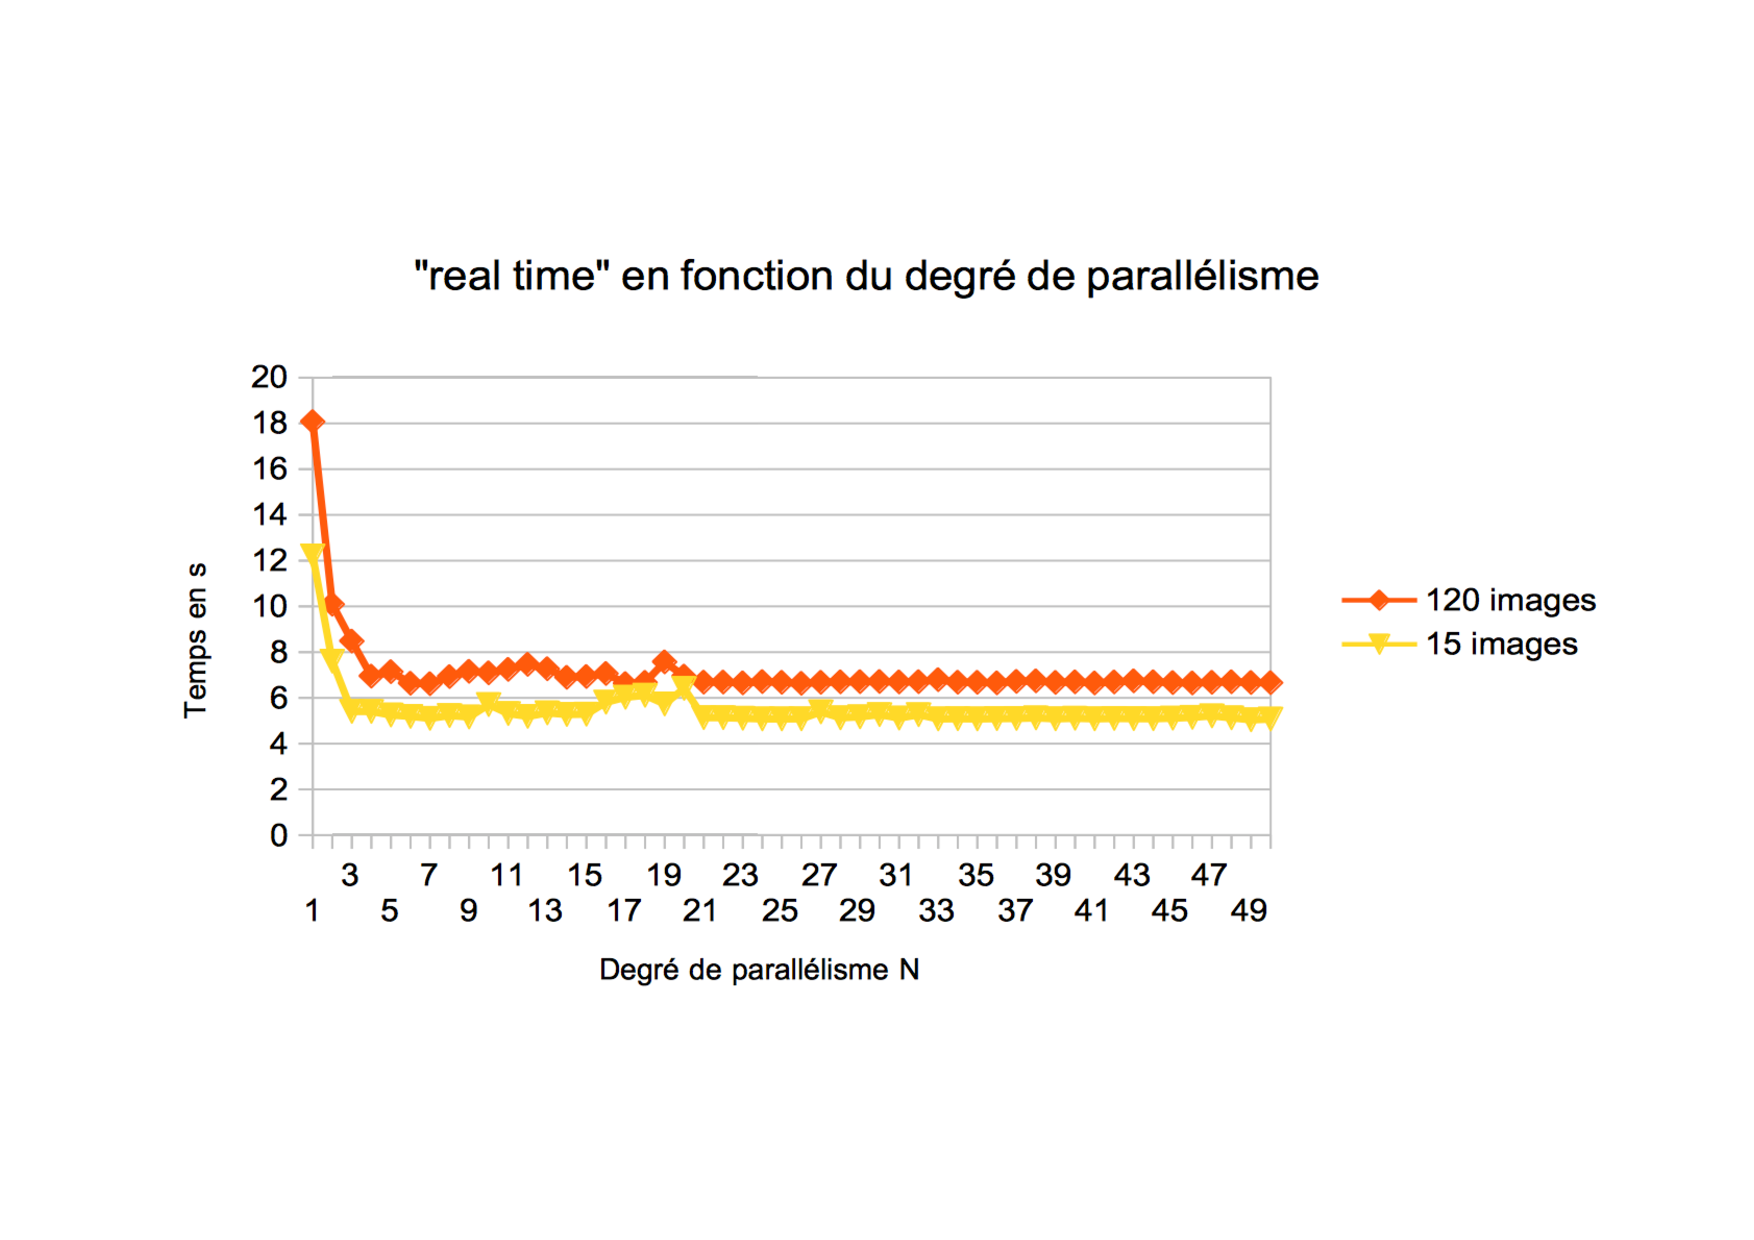
\includegraphics[width=12 cm]{time120-15chart_enhanced.pdf}
  \caption{Temps d'exécution de make en fonction du degré de
    parallélisme et du nombre d'images}
\end{center}
\label{fig:time_graph}
\end{figure}

\subsection{Correction du Makefile exiftags}Le problème avec le Makefile
exiftags était qu'il manquait un fichier de header dans la variable
\lstinline!HRDS!, ce qui signifie que si ce fichier était modifié, cela
n'aurait pas entrainé la recompilation du programme. Il a suffit de rajouter
\lstinline!timevary.h! à \lstinline!HRDS! pour palier au problème.

\end{document}
